\documentclass[10pt,a4paper,twocolumn]{article}
\usepackage[utf8]{inputenc}
\usepackage{amsmath}
\usepackage{amsfonts}
\usepackage{amssymb}


\usepackage{graphicx} 
\usepackage{subfigure}
\usepackage{paralist}
\usepackage[]{algorithm2e}
\usepackage{hyperref}
\usepackage{comment} %for anonymized version everything removed for anonymization is in \excludecomment{}


\usepackage{url}
\usepackage{booktabs}

\usepackage[usenames,dvipsnames]{xcolor}
\usepackage{tikz}
\usetikzlibrary{positioning, calc}

\usepackage[draft,nomargin,footnote]{fixme}

\graphicspath{{figs/}}

\usepackage{xspace}
\newcommand{\eg}{\textit{e.g.}\xspace}
\newcommand{\etal}{\textit{et al.}\xspace}
\newcommand{\ie}{\textit{i.e.}\xspace}
\newcommand{\etc}{\textit{etc.}\xspace}
\newcommand{\vs}{\textit{vs.}\xspace}

\begin{document}


\title{Mutual Modelling in Educational Child-Robot Interaction}


%\author{\# \# \#}
\author{Alexis Jacq$^{1,2}$\\
$^1$CHILI Lab, \'Ecole Polytechnique F\'ed\'erale de Lausanne, Switzerland,\\
$^2$GAIPS, Instituto Superior T\'{e}cnico, University of Lisbon, Portugal}




\maketitle
\begin{abstract}
In any constructive social interaction, agents must be able to understand each other. This mutual understanding requires the ability to establish a mental model of the other, called mutual modelling. My PhD is focused on mutual modelling in robotics: How robots can model other agents within social activities ? Such models must be dynamic in order to keep track of shared knowledge, and adaptive in order to deal with specific behaviours of agents. 
This work is directly applied to the Cowriter Project, that aims at exploring how a robot can help children with the acquisition of handwriting (http://chili.epfl.ch/cowriter). Does mutual modelling in robots would actually improve educative Human-Robot Interactions ?
\end{abstract}

\section{Introduction}
\subsection{Mutual Modelling in HRI}

When we grow up, we construct our knowledge through interaction. At the beginning we learn from parents language and basics of etiquette. Then we learn about culture, science and social behaviours at school with teachers, at work with colleagues or from family and friends. To make possible such a social learning, both learners and teachers need to model each others: a teacher has to be aware of understood knowledge of his student, and a learner has to take the perspective of his teacher to understand his lessons. 

Developed by Baron-Cohen [Baron-Cohen] and Leslie [Leslie], the Theory of Mind describes the ability to attribute mental states and knowledge to others. In interaction, humans are permanently collecting and analysing huge quantity of information to stay aware of emotions, goals and understandings of their fellows. In this work, we focus on a generalization of this notion to a more computational concept: the Mutual Modelling characterizes the effort of one agent to model the mental state of another one [dillenb. 1999]. 

We want to design a cognitive architecture that models mental states of different agents in interaction and that take decision from these models. We believe that to implement such an architecture in a robot will strongly improve human-robot interactions, making exchanges much more smooth and natural. 

\subsection{Application to the CoWriter project}
Children facing difficulties in handwriting integration are more exposed
to troubles during the acquisition of other disciplines as they grow up
\cite{Christensen2005}. 
The CoWriter activity introduces a new approach to help those children
\cite{Hood}. While common successful interventions involve children
in long intervention (at least 10 weeks) focused on \emph{motor} skills \cite{Hoy2011},
CoWriter is based on \emph{learning by teaching} paradigm and aims to repair
self-confidence and motivation of the child rather than his handwriting performance alone.

\emph{Learning by teaching} is a technique that engages students to conduct the activity in the role of the teachers in order to support their learning process. This 
paradigm is known to produce motivational, meta-cognitive and educational
benefits in a range of disciplines~\cite{Rohrbeck2003}. The CoWriter project
is the first application of learning by teaching approach to handwriting. 

The effectiveness of our learning by teaching activity is build on the
``prot\'eg\'e effect'': the teacher feels responsible for his student, commits
to the student's success and possibly experiences student's failure as his own
failure to teach. Teachable computer-based agents have previously been used to
encourage this prot\'eg\'e effect, where students invest more effort into
learning when it is for the benefit of a teachable agent than for themselves~\cite{Chase2009}.
We rely on this cognitive mechanism to reinforce the child's commitment into the
robot-mediated handwriting activity.

Our project requires a robot that play the role of a realistic learner to attract and challenge the child. At the moment, we have already implemented an tested the activity without mutual modelling ability in the robot [deana]: the movements, the learning curve and the sentences of the robot are set beforehand and do not depend on the interaction. But the realism of the learning robot and the prot\'eg\'e effect could be strongly improved if the robot was able to play his role according to a model of the child and, at a deeper level, to a model of \textit{the robot-perceived-by-the-child} and \textit{the child-perceived-by-himself}.

With a mutual modelling architecture, the robot could adapt his learning speed based on these models to make sure the child understands it is actually learning. Furthermore, we want a robot that implicitly leads the child to correct himself while correcting the robot: for example, it could detect and exaggerate the mistakes of the child. At another scale, the robot could have a physical behaviour adapted to the child: \textit{micro-behaviours} (small movements, gazes and sounds) must be based on the content of the interaction and on the behaviour of the child in order to improve the realism of the robot, to induce strong prot\'eg\'e effect and to make the interaction with the robot more comfortable for a young child. 

In this thesis, we aim to construct a general framework for mutual modelling and, in the same time, to develop and test it through this activity. We have designed an experimental framework that enable long-term studies in real pedagogic/therapeutic contexts [alexis]. Following this work, our results will be based on experimental studies with children that faces actual difficulties in learning. 

\section{Related work}


In several contexts, a various amount of fields have introduced their own framework to describe mutual modelling ability [severin \& pierre]. 
In Developmental psychology, Flavell [Flavell] names different levels of perspective taking from \textit{cognitive connection} (I see, I hear, I want, I like...) to \textit{representation} (what other agents feels, hear, want...). The study of a specific deficit, namely autistic spectrum disorder, led to develop the theory of mind through false-belief experiment [baron cohen][frith and happe], since this pathology is accompanied by a lake of theory of mind in affected children. 

In Psycholinguistics and collaborative learning, and more precisely in \textit{computer supported collaborative learning} (CSCL), Roschelle and Teasley [] suggested that collaborative learning has something to do with the process of constructing and maintaining a \textit{shared understanding} of the task at hand. 
At the beginning, the term ``mutual modelling" was introduced in this context, and was focused on the knowledge states of agents [pierre 1999].  Dillenbourg developed in [pierre 2014] a computational framework to represent mutual modelling situations. He introduced the notation \textbf{M(A,B,X)} to denote ``\textbf{A} knows that \textbf{B} knows \textbf{X}".

Epistemic logic uses another notation to describe a similar situation: $\textbf{K}_{\textbf{A}}\textbf{K}_{\textbf{B}}\textbf{X}$ where $\textbf{K}_{\textbf{i}}\textbf{X}$ stands for ``agent \textbf{i} knows \textbf{X} (see [epistemic logic] for overview and references). This notation has been extended to describe more complex situations like the \textit{shared-knowledge} (all the agents of a group know \textbf{X}) and the \textit{common-knowledge} (all the agent of a group know \textbf{X}, and know that all the agent know \textbf{X}, and know that all the agents know that all the agents know \textbf{X}..., etc.). 
However, Human-Robot Interaction research (HRI) has until now just scratched the surface. In [Scassellati], Scassellati gave an initial account of Leslie's and Baron-Cohen's theory of mind from the perspective of robotics, he limited his work to perceptual precursors (face detection or color saliency detection). Since then, some works (including Breazeal [breazeal], Trafton [trafton], Ros [ros] and Lemaignan [severin]) has been conduced to implement Flavell's first level of perspective taking [Flavell] (``\textit{I see (you do not see the book)}"), ability that is limited to the process of visual perception.
In [withmeness], Lemaignan implemented a system that compute in real time the visual field of agents and estimate which objects are looked. This time, the robot is not just aware of what \textit{can be seen} by agents, but it perceives what \textit{is currently looked}. Lemaignan used this device to measure Sharma's \textit{with-me-ness}~\cite{sharma2014me} within the CoWriter activity, as the quantity of time the child looks what he is expected to look according to the current task/event. His results provided by the algorithm were significantly close to human's perception of the \textit{with-me-ness}.


\section{CoWriter: description of the activity}
\subsection{Interaction overview}
Figure~\ref{experimental_setup} illustrates our general experimental setup: a
face-to-face child-robot interaction with an (autonomous) Aldebaran's {\sc nao}
robot.

A tactile tablet (with a custom application) is used by both the robot and the
child to write: in each turn, the child requests the robot to write
something (a single letter, a number or a full word), and pushes the tablet
towards the robot, the robot writes on the tablet by gesturing the writing (but
without actually physically touching the tablet). The child then pulls back the
tablet, corrects the robot's attempt by writing himself on top or next to
the robot's writing (see Figure~\ref{fig:Vincent}), and ``sends'' his
demonstration to the robot by pressing a small button on the tablet. The robot
learns from this demonstration and tries again.

Since the child is assumed to take on the role of the teacher, we had to ensure
he would be able to manage by himself the turn-taking and the overall
progression of the activity (moving to the next letter or word). In our design,
the turn-taking relies on the robot prompting for feedback once it is done with
its writing (simple sentences like ``What do you think?''), and pressing on a
small robot icon on the tablet once the child has finished correcting. We found that both approaches were easy to grasp for children.


   \begin{figure}
       \centering
       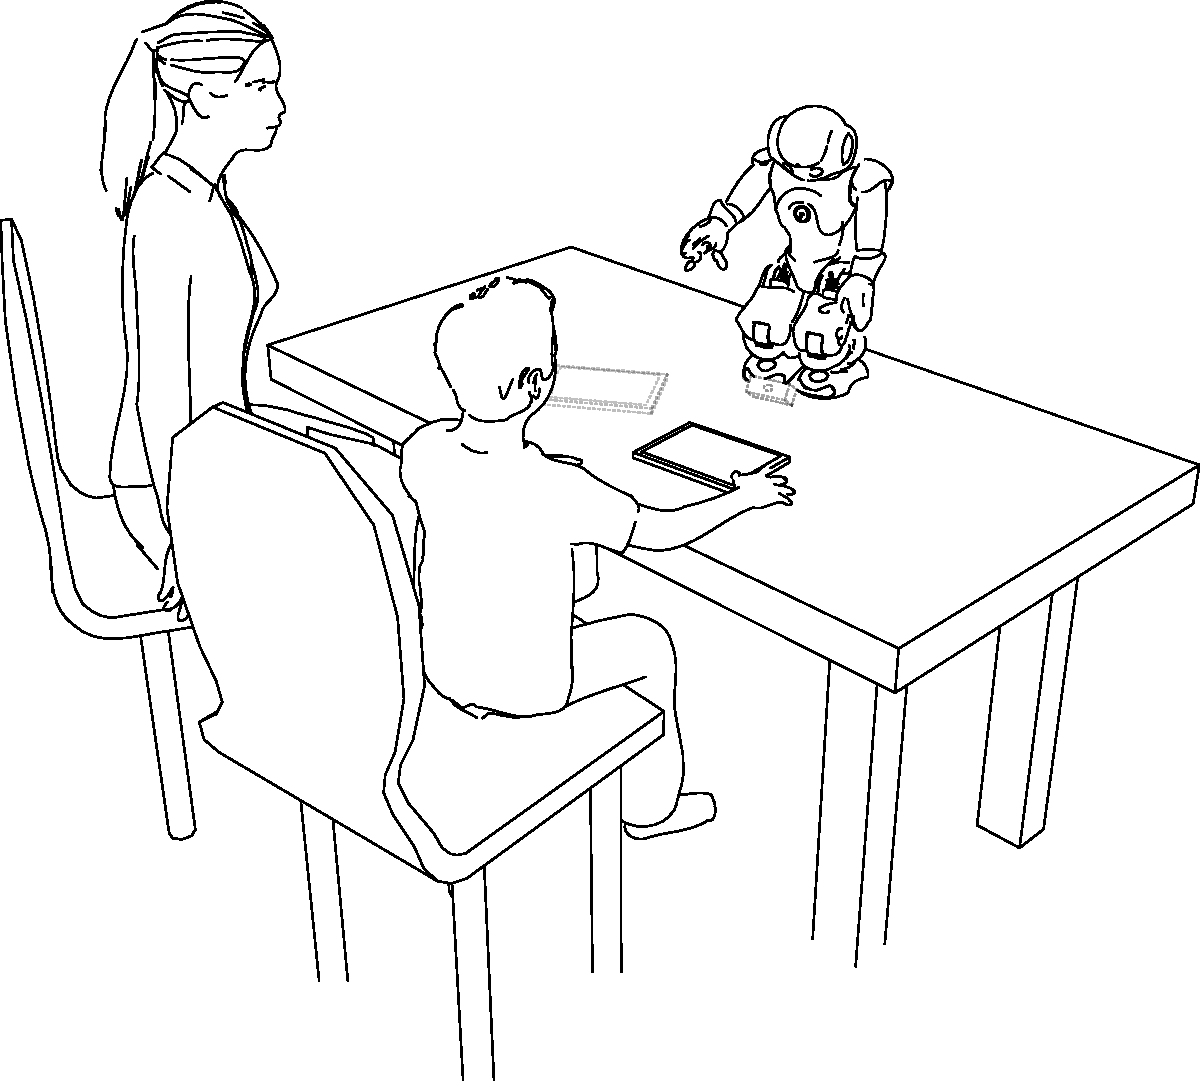
\includegraphics[width=0.6\columnwidth]{experimental_setup}
       \caption{\small Our experimental setup: face-to-face interaction with a {\sc
           nao} robot.  The robot writes on the tactile tablet, the child then
           corrects the robot by directly overwriting its letters on the tablet
           with a stylus. An adult (either a therapist or an experimenter,
           depending on the studies), remains next to the child to guide the work
           (prompting, turn taking, etc.). For some studies, a second tablet and an
           additional camera (lightened) are employed.}

       \label{experimental_setup}
   \end{figure}
   
In [alexis], we added buttons to the tablet interface to allow the child to evaluate the robot. Even if this feedback does not necessary concerns the progress of the robot's writing (children also use them to express how they like the robot), we can still exploit and improve this idea to get effective information about the child's perception of the robot.
   
The robotic implementation of this activity is explained in [Deana]. We used ROS to ensure the synchronization and communication between different devices. Likewise, the cognitive architecture for mutual modelling will be deigned as a ROS module that will collect information about the mental state of agents (here, the child, or \textit{the robot-perceived-by-the-child}, or \textit{the child perceived by the himself}) in order to update its model of these agents. Then, other modules (for example the module that govern the learning algorithm of the robot) will use these models to make decisions. We will better explain this design below, in section [cognitive architecture / implementation].

\subsection{Generating and learning letters}

Since our approach is based on teaching a robot to write, generating (initially
bad) letters and learning from demonstrations is a core aspect of the project.
The initial state of the robot and his ability to learn in an obvious way
from demonstrations of the child is the key to lend credibility to the activity and to induce the ``prot\'eg\'e" effect.

The technical idea is simple: allographs of letters are encoded as a sequence of 70 points in
2D-space and can be seen as vectors with 140 elements
($x_1,...,x_{70},\hspace{1mm}y_1,...,y_{70}$). We arbitrary chose a set of allograph
that define the initial state of generated letters. 
After the child provided a demonstration of a letter, the algorithm
generates a new letter corresponding to the middle point between the last state and the
demonstration. Details of this algorithm are presented in [deana] and [alexis].

However, to keep the child engaged, the robot must learn at the right rate, not too fast otherwise the kid will have
no opportunity for improving his skills and not too slow otherwise he may loose
trust in his ability to improve the robot' skills. And a learning curve just based on the middle point between last state and demonstration will be too fast for one child, and too slow for another one. We need to make the robot aware of the child's perception of it progresses to take decision about its own learning curve. This awareness should be taken in account in our mutual modelling implementation, described below. 


\section{Framework for mutual modelling in robotics}

\subsection{Definitions}
In this work, we extend the definition of mutual modelling from the representation of knowledge states to more global agent's states including knowledges but also positions, behaviours, emotions, beliefs, desires, pretending... etc. 

In order to enable second-order theory of mind (the ability to attribute a theory of mind to other agents), we define two order of agents: the \textit{first-order-agents} concerns direct representations of agents by the robot (for example the child), while the \textit{second-order-agents} concerns the representation of agents by agents (for example the robot-perceived-by-the-child). To model second-order-agent like the robot-perceived-by-the-child is crucial if we want to play with the perception of the robot, e.g. to make sure the child understand that the robot is learning from his demonstrations. We can as well define \textit{$n^{\textit{th}}$-order} agents to play with higher level of theory of mind. In our implementation applied to the CoWriter activity, we will just use the two first orders. Unlike the epistemic logic, our framework will not take into account infinite loops of mutual modelling (as does the \textit{common-knowledge} operator \textbf{CK} described in related works). 

The sensitive devices (for example cameras, micros, tactile sensors... and in the case of CoWriter the tablet's inputs) are used to measure a quantity of \textit{perceived variables} (the position in space of agents, the gaze targets, quality of demonstrations, the time to respond, the evaluation of the robot by the child...). Each \textit{perceived variable} is associated to the model of one agent (in CoWriter, the positions in space of the child is associated to the model of the child, while the evaluation of the robot is associated to the model of the child-perceived-by-the-robot). 

We define two levels of perceived variables: the \textit{internal}, describing mental states (knowledges, beliefs, emotions, goals...), and the \textit{external}, describing the physical states (position in space, micro-behaviours, focus of attention, amount of movement...). These two levels are fundamentally different but closely dependent: if an agent is looking in a wrong direction during a demonstration, it will not assimilate the knowledge that it is provided. Reversely, if an agent understand a new knowledge from a demonstration or feels a strong emotion, its behaviour will be directly affected in consequence. We will use some trivial assumption about these dependency to make prediction about understanding and expected micro-behaviours (see the section [dynamics]).

A model of an agent is the set of all the values of the perceived variables associated to this model. It can be formalized by two vectors: one for the values of internal variables and one for external variables. Since the values of the perceived variables are likely to change with the time, the models are dynamic.

\subsection{Notations}

The notation introduced by Dillenbourg in [dillen. 2014] is effective to describe complex multi-agent situations, but becomes quickly heavy when it is used for second-order mutual models: if \textbf{C} stands for the child and \textbf{R} for the robot, the model of the child-perceived-by-the-robot would be written \textbf{M(R; C; M(C; R; . ))}.

In a context of HRI, most of the time we will consider one robot modelling human agent(s). Hence, we can assume that all the mutual models are processed by the robot. We will denote $\textbf{M}_\textbf{A}$ the model of an agent $\textbf{A}$, and $\textbf{M}_\textbf{AB}$ the model of the agent-\textbf{B}-perceived-by-the-agent-\textbf{A}. With this notation, the child-perceived-by-the-robot is described by $\textbf{M}_\textbf{CR}$. In the rare cases of the usage of more than one robot, the model processed by different robots can be distinguished by an additive index ($\textbf{Mi}_\textbf{A}$ describing the model of the agent \textbf{A} by the robot \textbf{i}). Models of third and higher orders agent are noted as well with a sequence of agent: $\textbf{M}_\textbf{ABCD}$ stands for ``((\textbf{A} \textit{perceived by} \textbf{B}) \textit{perc. by} \textbf{C}) \textit{perc. by} \textbf{D}".

If $x^t$ represents the value of a perceived variable $X$ at time $t$, We can see the model of an agent \textbf{A} as a mapping $\textbf{M}^t_\textbf{A}: X \mapsto x^t$ that provides the value of the associated variables. 








\section{Cognitive architecture}

\section{Experimental studies}

\section{Next steps}

\section{Conclusion}



\bibliographystyle{abbrv}

\bibliography{cowriter} 

\end{document}
